\documentclass[12pt]{article}
\usepackage[top=1in, bottom=1in, left=1in, right=1in]{geometry}
\usepackage[justification=centering]{caption}
\usepackage{graphicx}
\usepackage{listings}
\usepackage{color}
\usepackage{indentfirst}
\usepackage{hyperref}
\usepackage{siunitx}
\usepackage{float}
\usepackage{amsmath}

\lstset{ %
	%language=C,                % choose the language of the code
	basicstyle=\scriptsize,       % the size of the fonts that are used for the code
	                  % how far the line-numbers are from the code
	backgroundcolor=\color{white},  % choose the background color. You must add \usepackage{color}
	showspaces=false,               % show spaces adding particular underscores
	showstringspaces=false,         % underline spaces within strings
	showtabs=false,                 % show tabs within strings adding particular underscores
	%frame=single,           % adds a frame around the code
	tabsize=2,          % sets default tabsize to 2 spaces
	captionpos=b,           % sets the caption-position to bottom
	breaklines=true,        % sets automatic line breaking
	breakatwhitespace=false,    % sets if automatic breaks should only happen at whitespace
	escapeinside={\%*}{*)}          % if you want to add a comment within your code
}

\begin{document}
\title{Microprocessor Systems\\ Lab 6: Memory Interfacing }
\author{Nick Choi \and Samuel Deslandes}
\date{12/05/16}
\maketitle
\pagebreak
\section{Introduction}
The overall goal of this lab was to become familiar with configuring the 8051 to utilize an LCD display and a keypad. 

In the first section of the lab, a C program was written to create the user interface for the magic 8 ball through the ANSI terminal. The interface consists of four generic questions that the user can select in order to receive a randomized answer form the 8051. These questions include “Yes/No” questions, “True/False” questions, “Days of the week questions”, and lastly, “random number” questions. The questions could be selected by entering the appropriate keys on the keyboard connected to the ANSI terminal.  

In the second section of the lab, the C program developed for section 1 was modified so that the user could see the answers to their questions on a LCD display. The answers to the user’s questions are displayed on the screen until a new answer is generated by the magic 8 ball. 

In the third section of the lab, the C program used in sections 1 and 2 was further modified to incorporate a keypad as the means of user input rather than using a keyboard. In order for the keypad to function properly, a digital logic circuit was constructed in order to properly trigger an external interrupt on the 8051. Additionally, the output of the keypad needed to be decoded by the 8051 to properly determine which button on the keypad was pressed. 


\section{Methods}
\subsection{Software}
The code for parts 1, 2 and 3 can be found in Appendix A, B and C respectively. All code was uploaded and run on the 8051 through the programming/debugging USB port. 

\subsubsection{Part 1}
In the first section of this lab an electronic ``Magic 8 Ball'' was developed. The program generates responses to four types of questions that can be asked:
	\begin{itemize}
		\item Yes/No
		\item True/False
		\item Day of the week
		\item Random Number
	\end{itemize}

In order to randomly select a response, Timer0 is is configured to continuously count, and is sampled when a response is required. Timer0 was configured as a 16-bit timer by setting the lower nibble of the TMOD SFR to \texttt{0x01}. Although Timer0 is a 16-bit timer, only the lower byte (stored in TL0) is sampled. The timer was also configured to use SYSCLK/12 as a base by clearing bits 0, 1, and 3 of the CKCON SFR. 

When configuring ports, bits 0--3 of port 3 should be configured as inputs, and bits 4--7 as outputs. This is done by setting the `P3MDOUT' SFR to \texttt{0xf0}, and the `P3' SFR to \texttt{0x0F}.

In the main function, user input is retrieved using the getchar() function. A switch/case block is then used to handle the user input and generate the appropriate response. In the case of a binary response, such as for the `Yes/No' or `True/False' questions, TL0 is read and modded by 2. The result is then evaluated to be either 1 or 0 and a response is printed to the terminal accordingly. 

To handle the `Days of the week' question an array of strings declared as ``const char*'' was used to store each day of the week. The value held in TL0 is then modded by 7 and used to index the aforementioned array. In order to print the string, `printf()' was used with the `\%s' formatting keyword. 

To handle the `Random number' question case, first the user must be prompted for max and min values to designate a range of responses. This is done using `getchar()'. To randomly select an integer within this range the following equation is used:
\begin{displaymath}
\text{min+TL0\%(max-min+1)}
\end{displaymath}
The right side of the equation produces a number within the difference of the max and min values selected; adding the minimum value to this brings it back within the range. 

In addition to the four cases corresponding to the types of questions that can be asked, there is also the default case, which is triggered when the input is invalid. In this case the program notifies the user of the invalid input and waits for the next user input. 

\subsubsection{Part 2}
The code for this section of the lab is an enhancement of the previous part, which prints output not only to the terminal, but also to an LCD screen. In order to print to the LCD screen, first the ``LCD.h'' and ``LCD.c'' files must be included; these files contain the functions ``lcd\textunderscore clear()'' and ``lcd\textunderscore puts()'' which are used to clear the LCD and write to the LCD respectively, as well as the ``lcd\_init()'' function used to initialize the LCD. As mentioned before, the code for this section is the same as that of the previous section, with the addition of the ``lcd\_init()'' function called together with the other init functions, and clearing the LCD and printing to it after printing to the terminal when outputting responses. 

\subsubsection{Part 3}
The code for this section further enhances that of the previous section by using a keypad to receive user input, rather than the keyboard. The keypad is wired such that when a key is pressed, an external interrupt (/INT0) is triggered. To do this, /INT0 must be routed to port pin P0.2, which is done by setting bit 2 of the XBR1 SFR. Next, global interrupts and /INT0 must be enabled, which can be done using the bit-addressable variables `EA' and `EX0' respectively. 

%talk about key wakeup and decoding
Once /INT0 has been triggered, the associated ISR must decode the signals on port 3 to determine which key has been pressed. The ISR starts by setting `EX0' to 0, disabling interrupts on /INT0. Next, a flag variable is set, and the lower nibble of P3 is stored in a variable called ``keyvalue'' for use in decoding columns. This is done using a bitwise AND operation between P3 and \texttt{0x0F}.

At this point the rows can be decoded. To check if a key in the top row was pressed, P3 is set to \texttt{0x8F}, and after a short pause the lower nibble of P3 is evaluated. If it evaluates to \texttt{0x0F}, this is the row that was selected, and the ISR moves on to decode the columns. If this is not the case, then this process is repeated setting P3 to \texttt{0x4F}, \texttt{0x2F}, or \texttt{0x1F} for each of the subsequent rows. 

Decoding columns is done by simply evaluating the ``keyvalue'' variable declared before the row decoding to determine which bit in its lower nibble has a value of 0. This is done using the comparison operator with the values \texttt{0x07}, \texttt{0x0B}, \texttt{0x0D}, and \texttt{0x0E} corresponding to the columns of the keypad from left to right. Once the selected column has been identified, a character can be assigned to a global variable ``asciichar'' for use in the main function. Figure \ref{KEY} in the appendices section can be used as a reference for which row and column intersection corresponds to what character. 

Once ''asciichar`` has been assigned P3 is reset to \texttt{0x0F}, and after another pause /INT0 is re-enabled and the program returns from the ISR.  

In the main function, rather than using `getchar()' to get user input, a new function ``getkeychar()'' was written. This function waits for the flag variable set in the /INT0 ISR to go high, resets the flag, then returns the ``asciiflag''. The rest of the main algorithm is the same as it was in the previous section.  

\subsection{Hardware}
The hardware for this lab involved interfacing the 8051 with a LCD screen in part 2, and a keypad in part 3.

\subsubsection{Part 1}
No hardware was required for this section.

\subsubsection{Part 2}
In this section a LCD screen was wired to the 8051. A schematic for this can be viewed in Figure \ref{LCD} in the appendices section below. The LCD module used for this lab had 14 pins.
Pins 1 and 2 are connections to ground and power, respectively. Pin 3 controls the screen contrast, which can be controlled using a potentiometer which comes as a part of the module. Pins 4, 5, and 6 are the register select, read/write select, and enable control signals, which were connected to P7.0--P7.2 on the 8051. Since port 7 was left in open-drain mode, a 10k\si{ohm} pull-up resistor was placed between P7.2 and power. Pins 7 to 14 are data pins, which were connected to all of port 6 on the 8051. Port 6 should be configured as open-drain with high-impedance on every pin. This does not have to be done explicitly in the code because this can be accomplished using the associated SFRs' default values.

\subsubsection{Part 3}
In this section a keypad was wired to the 8051. A schematic can be viewed in Figure \ref{KEY} in the appendices section below. The keypad requires 8 wires, 4 for the columns and 4 for the rows, each of which are connected to port 3 on the 8051. The columns are connected to the lower nibble of port 3 (P3.0--P3.3) which is configured as open-drain for input. These wires are held high using a 3.3\si{V} and 10k\si{\ohm} pull-up resistors, and are also used as inputs to a four input and gate. The output of this gate is used as the /INT0 interrupt source and is connected to pin 2 of port 0 (P0.2). The rows are connected to the high nibble of port 3 (P3.4--P3.7), which is configured as push-pull for output. These wires are held low by the software. 

\section{Results}
By completing section one of the lab, a C program was developed that would create a user interface for the magic 8 ball using the ANSI terminal. By completing section two of the lab, a C program was developed to send the magic 8 ball’s answers to a LCD display. By completing section three of the lab, a C program was developed in order to interface a keypad with the magic 8 ball. The keypad replaced the keypad input and a glue logic circuit was constructed in order to properly interface with the keypad. 	


\section{Conclusion}
Our end results matched well with the general goals for this lab however there were several instances where the system did not perform as expected. In section two of the lab, the messages that were being displayed on LCD would sometimes become corrupted. It was determined that this was the case because the display was not given enough time to properly output the entire message. 

In section three of the lab, the terminal was randomly receiving duplicate button presses. The cause of this issue was that the keypad was not being sufficiently debounced. Therefore, the software debouncing period was increased in order to filter unintended button presses. Another approach to this issue could have been to implement a hardware debouncing circuit using logic gates or a simple RC circuit. 
 


\section{Appendices}
\subsection{Modified putget.h}
\lstinputlisting{putget.h}

\subsection{Part 1}
\subsubsection{Code}
	\lstinputlisting{part1.c}
\subsection{Part 2}
\subsubsection{LCD Schematic}
\begin{figure}[H]
	\centering
	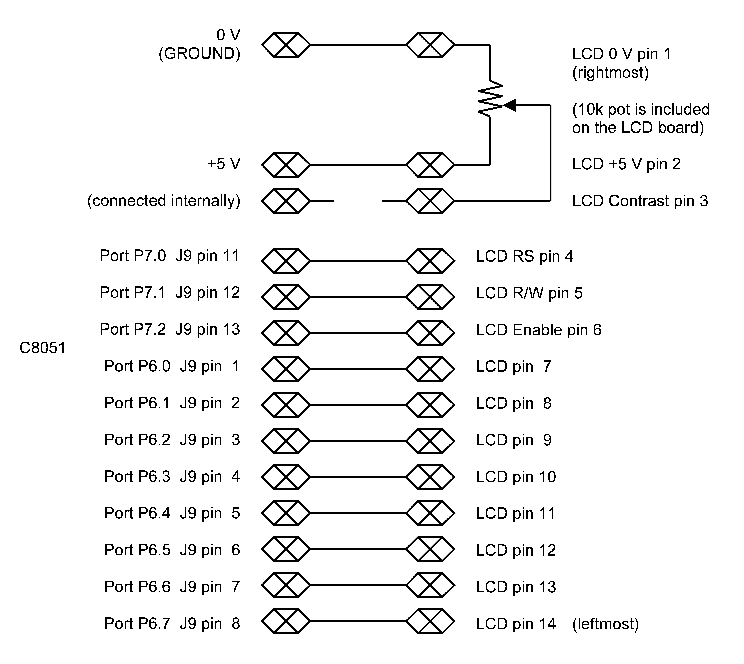
\includegraphics[width=\textwidth]{lcd_schematic.png}
	\caption[]{Circuit schematic for LCD[2]}
	\label{LCD}
\end{figure}

\subsubsection{Code}
	\lstinputlisting{part2.c}	
\subsection{Part 3}
\subsubsection{Keypad Schematic}
\begin{figure}[H]
	\centering
	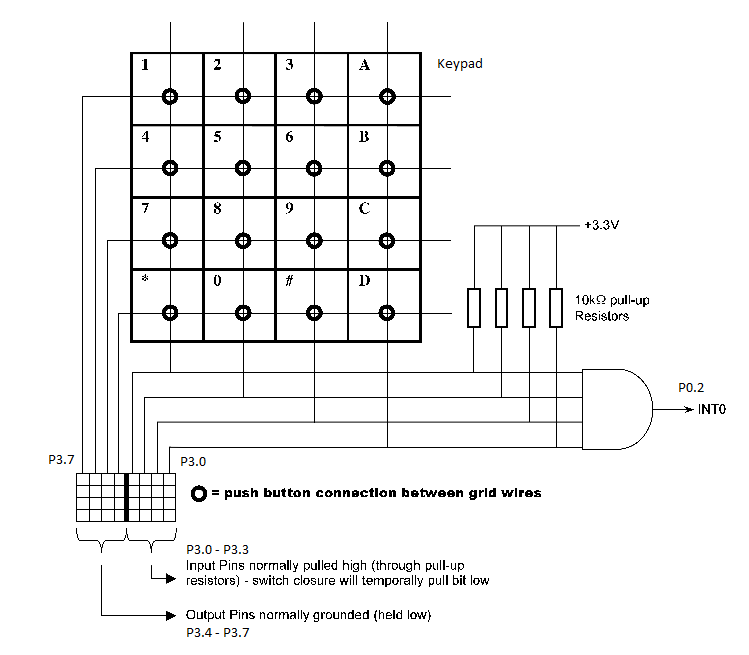
\includegraphics[width=\textwidth]{keypad_schematic.png}
	\caption[]{Circuit schematic for keypad[1]}
	\label{KEY}
\end{figure}
\subsubsection{Code}
	\lstinputlisting{part3.c}

\section{References} 
\noindent
[1]``MPS Lab 6," in RPI ECSE Department, 2016. [Online]. Available: \url{http://www.rpi.edu/dept/ecse/mps/MPS_Lab_Ex6-Magic8Ball.pdf}. Accessed: Nov. 27, 2016.\\
\newline\noindent
[2]``Interfacing a Hitachi HD44780 to a Silicon Laboratories C8051F120," in RPI ECSE Department, 2016. [Online]. Available: \url{http://www.rpi.edu/dept/ecse/mps/LCD_Screen-8051.pdf}. Accessed: Nov. 27, 2016.\\
\newline\noindent
[3]``C8051 Manual," in RPI ECSE Department, 1.4 ed., 2005. [Online]. Available: \url{https://www.ecse.rpi.edu/courses/CStudio/Silabs/C8051F12x-13x.pdf}. Accessed: Nov. 27, 2016.


\end{document}